% !TEX root = ../main.tex
\chapter{Introduction}
\label{chapter:Introduction}

% TODO notes:
% Check name of professor Uni Prof Dr. Ing
% Change sectioning to keep all on one ground 3.1 3.2
% Change all literature to be non arxiv form
% Add the code consent section
With the continued advancements of artificial intelligence, the interest in self-navigating autonomous robots has dramatically increased, reflecting their growing role as a safe and efficient solution for traversing complex industrial environments \cite{keith_review_2024, zghair_one_2021, loganathan_systematic_2023}.
Furthermore, vehicle manufacturers are now extending this interest to the consumer market with the development of fully Autonomous Vehicles (AVs) \cite{hu_review_2026}.
Companies such as Waymo and Baidu already operate fully autonomous taxi services in a number of cities in the United States and China \cite{hu_review_2026, jain_Autonomy_20_2021}.
Several announcements have also indicated that these services will extend to European countries such as England, Switzerland, and Luxembourg \cite{saether_recommendations_2026}.
Unfortunately, as revolutionary as autonomous mobile robots are, they are not without their flaws \cite{jain_Autonomy_20_2021, hu_review_2026}.
These flaws often stem from the two main architectural structures that researchers utilize to develop and train the autonomous driving algorithms for these vehicles: the modular architecture and the end-to-end neural network architecture \cite{jain_Autonomy_20_2021,jahncke_MINDStackModularInterpretable_2025, huang_DifferentiableIntegratedMotion_2024, karkus_DiffStackDifferentiableModular_2022}.

The modular architecture, also called a modular stack, relies on imposing human-written rules to dictate the vehicle's behavior \cite{hu_review_2026, jain_Autonomy_20_2021, jahncke_MINDStackModularInterpretable_2025, tampuu_SurveyEndtoEndDriving_2022, wang_VersatileEfficientReinforcement_2022}.
As seen in Figure \ref{fig:modulararch}, the stack generally consists of interconnected functional units.
%? include this part or don't
%? A robot that is completely autonomous is able to observe its surroundings, make judgments based on what it sees and/or has been trained to recognize, and then carry out an action or manipulation in that environment. 
The perception unit interprets the vehicle's surroundings with the use of the sensor data to be used for prediction \cite{ogretmen_local_2025, hu_review_2026}.
The prediction unit then estimates future states based on an end goal, such as predicting the paths of surrounding cars in traffic.
Using this forecast, the planning unit computes a trajectory that the ego vehicle can safely follow.
Ultimately, the control unit takes this trajectory and sends commands to the car.

\begin{figure}[hb]
    \centering
    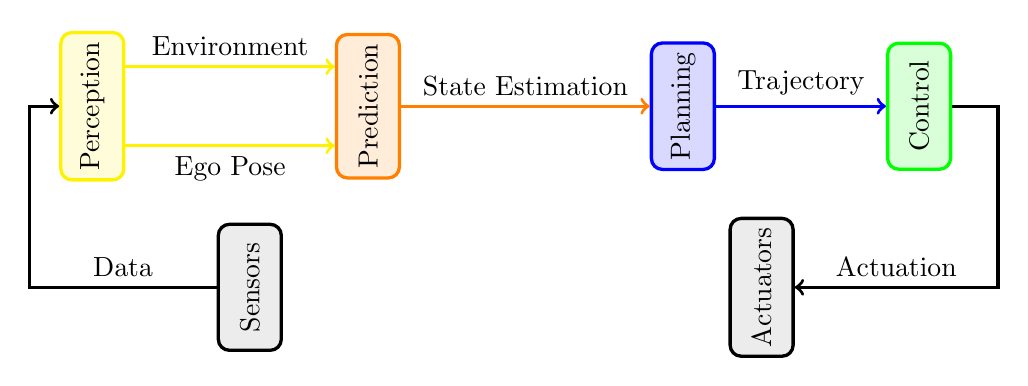
\begin{tikzpicture}
        \node[name=sensors, shape=rectangle, draw=black, fill=gray!15, very thick, rounded corners, minimum width=1.6cm, minimum height=0.8cm, rotate=90] at (4,-2.3) {Sensors};
        \node[name=perc, shape=rectangle, draw=yellow, fill=yellow!15, very thick, rounded corners, minimum width=1.6cm, minimum height=0.8cm, rotate=90] at (2, 0) {Perception};
        \draw[->, black, very thick] (sensors.north) -- node[midway, above] {Data} (1.2, -2.3) -- (1.2, 0) -- (perc.north);
        \node[name=pred, shape=rectangle, draw=orange, fill=orange!15, very thick, rounded corners, minimum width=1.6cm, minimum height=0.8cm, rotate=90] at (5.5, 0) {Prediction};
        \draw[->, yellow, very thick] (perc.320) -- node[midway, above, black] {Environment} (pred.40);
        \draw[->, yellow, very thick] (perc.220) -- node[midway, below, black] {Ego Pose} (pred.140);
        \node[name=plan, shape=rectangle, draw=blue, fill=blue!15, very thick, rounded corners, minimum width=1.6cm, minimum height=0.8cm, rotate=90] at (9.5, 0) {Planning};
        \draw[->, orange, very thick] (pred.south) -- node[midway, above, black] {State Estimation} (plan.north);
        \node[name=ctrl, shape=rectangle, draw=green, fill=green!15, very thick, rounded corners, minimum width=1.6cm, minimum height=0.8cm, rotate=90] at (12.5, 0) {Control};
        \draw[->, blue, very thick] (plan.south) -- node[midway, above, black] {Trajectory} (ctrl.north);
        \node[name=act, shape=rectangle, draw=black, fill=gray!15, very thick, rounded corners, minimum width=1.6cm, minimum height=0.8cm, rotate=90] at (10.5,-2.3) {Actuators};
        \draw[->, black, very thick] (ctrl.south) -- (13.5, 0) -- (13.5, -2.3) -- node[midway, above] {Actuation} (act.south);
    \end{tikzpicture}
    %* fix citation
    \caption{An example of a possible implementation of the modular architecture for autonomous vehicles. Functional modules are shown in color (perception in yellow, prediction in orange, planning in blue, control in green) and vehicle hardware in grey. Inspired by \cite{ogretmen_local_2025}.}
    \label{fig:modulararch}
\end{figure}

\newpage
On the one hand, this modular pipeline offers a highly interpretable information path for the engineer.
It facilitates modifying the underlying behavior of the vehicle and ensures developers robustly implement well-defined safety measures \cite{jain_Autonomy_20_2021, jahncke_MINDStackModularInterpretable_2025, karkus_DiffStackDifferentiableModular_2022, tampuu_SurveyEndtoEndDriving_2022, wang_VersatileEfficientReinforcement_2022}.
On the other hand, these rule-based systems depend heavily on experts who must continually formulate new rules to optimize the stack's overall cost function \cite{jain_Autonomy_20_2021, karkus_DiffStackDifferentiableModular_2022, wang_VersatileEfficientReinforcement_2022}.
Because these systems are inherently unable to generalize effectively, encountering edge cases or expanding operations into new locations necessitates extensive re-tuning.
This limitation introduces substantial scaling bottlenecks \cite{hu_review_2026, jain_Autonomy_20_2021, huang_DifferentiableIntegratedMotion_2024, karkus_DiffStackDifferentiableModular_2022}.
Furthermore, evaluating the vehicle's performance solely through offline simulators does not provide an accurate representation of real-world conditions.
Consequently, development teams must perform extensive on-road testing, which exacerbates the scalability bottlenecks even further \cite{jain_Autonomy_20_2021}.
While such an approach can achieve high levels of reliability within carefully engineered scenarios, the aforementioned restrictions make purely modular architectures difficult to deploy economically across mass-produced autonomous vehicle fleets.

Alternatively, the end-to-end neural network architecture replaces the entire modular stack with a single learned model.
It takes raw sensor data from the vehicle and outputs its best prediction for the ego vehicle's course of action \cite{jain_Autonomy_20_2021, karkus_DiffStackDifferentiableModular_2022, tampuu_SurveyEndtoEndDriving_2022,wang_VersatileEfficientReinforcement_2022, kocic_end-to-end_2019, lee_autonomous_2020, hu_learning_2021}.
The commonly used learning paradigms, such as Imitation Learning (IL) or Reinforcement Learning (RL), are used to train the network and gradually improve its predictions \cite{hu_review_2026, huang_DifferentiableIntegratedMotion_2024, karkus_DiffStackDifferentiableModular_2022, ogretmen_local_2025, tampuu_SurveyEndtoEndDriving_2022, wang_VersatileEfficientReinforcement_2022, moller_LearningSampleReinforcement2025}.
This training leverages large datasets and significant computational resources, mitigating the scalability issues faced by modular stacks and allowing the resulting models to generalize their behavior to previously unencountered scenarios \cite{jain_Autonomy_20_2021, tampuu_SurveyEndtoEndDriving_2022, wang_VersatileEfficientReinforcement_2022}.
Unfortunately, achieving commercial-ready performance for autonomous vehicles requires extensive sensor data collection, preprocessing of the data, and the subsequent computationally intensive training of the neural network \cite{kocic_end-to-end_2019, lee_autonomous_2020, hu_learning_2021}.
Another drawback of neural networks is that their learned decision-making process remains largely unknown, as they are often described as mathematical black boxes whose internal reasoning is difficult to interpret \cite{hu_review_2026, jain_Autonomy_20_2021, jahncke_MINDStackModularInterpretable_2025, tampuu_SurveyEndtoEndDriving_2022, wang_VersatileEfficientReinforcement_2022}.
This lack of transparency conflicts with implementing explicit safety constraints and traffic regulations \cite{hu_review_2026, huang_DifferentiableIntegratedMotion_2024, karkus_DiffStackDifferentiableModular_2022, tampuu_SurveyEndtoEndDriving_2022, wang_VersatileEfficientReinforcement_2022}.
Consequently, although end-to-end models exhibit strong generalization capabilities, their unpredictability and limited interpretability present a significant hurdle for the safe deployment of consumer autonomous vehicles.

A middle-of-the-road approach that combines the modular stack with an end-to-end neural network is now gaining traction in the literature \cite{jahncke_MINDStackModularInterpretable_2025, huang_DifferentiableIntegratedMotion_2024, karkus_DiffStackDifferentiableModular_2022, wang_VersatileEfficientReinforcement_2022, swadiryus_DifferentiableMotionPlanning_2025, koch_DifferentiableInterpretablePath_2025}.
This hybrid approach retains the structure and interpretability of modular pipelines while integrating the learnable components of a neural network.
The goal of this method is to achieve an end-to-end differentiable hybrid stack, where gradients from downstream task-specific losses can be backpropagated through intermediate modules.
Hence, upstream components are trained to improve the overall performance of the model rather than performing a local optimization of each unique module.
Examples of this architecture in an urban scenario include the works of Huang et al. \cite{huang_DifferentiableIntegratedMotion_2024} and Karkus et al. \cite{karkus_DiffStackDifferentiableModular_2022}, which demonstrate that joint gradient-based optimization outperforms stacks of individually optimized modules.
Additionally, Jahncke and Betz \cite{jahncke_MINDStackModularInterpretable_2025} describe the Modular, Interpretable, and Differentiable (MIND) software stack, which applies the same principle of co-optimizing differentiable localization and control modules on the RoboRacer platform.

Building on MIND, Swadiryus \cite{swadiryus_DifferentiableMotionPlanning_2025} extended the RoboRacer stack with DiffPlan, a differentiable local planner that augments MIND's fixed global raceline with online local trajectory generation.
Specifically, Swadiryus \cite{swadiryus_DifferentiableMotionPlanning_2025} developed a trajectory-sampling planner, which generates a series of finite-horizon trajectories and scores them based on a cost function.
The planner then selects the trajectory with the smallest cost to be passed to the control unit.
Later, Koch \cite{koch_DifferentiableInterpretablePath_2025} relaxed the discrete selection of a candidate trajectory with a differentiable sample-selection method, connecting planner output to downstream control through end-to-end loss terms.
DiffPlan showed that gradients from downstream control objectives can propagate back through the planner to co-train localization and learnable cost weights for autonomous racing.
Unfortunately, deploying DiffPlan on the physical RoboRacer vehicle revealed unstable real-time operation due to computational inefficiencies \cite{koch_DifferentiableInterpretablePath_2025}.

Accordingly, this thesis aims to enable on-board computation of the entire DiffPlan stack so that the RoboRacer vehicle can run independently.
This is achieved through computational optimizations such as vectorization, just-in-time (JIT) compilation, and precomputation of static data.
Additionally, this thesis investigates an alternative local-motion-planning method that uses spatial sampling to generate an online velocity profile.
A series of experiments will be conducted to measure the speedup achieved by the optimized algorithms and benchmark the two differentiable local motion planners against each other: The temporal sampler DiffPlan and the spatial sampler DiffSpatialPlan.

Part \ref{part:stateoftheart} presents the literature review of past and current methods of autonomous vehicle systems in Chapter \ref{chapter:AutonomousDrivingSystems}.
%? to the mathematical foundations to describe the workings of motion planners and the subsequent branch of differentiable motion planners.
In addition, the state-of-the-art methods of motion planners, which allow autonomous navigation of vehicles, are discussed in Chapter \ref{chapter:MotionPlanners}.
The part concludes with Chapter \ref{chapter:DiffPlan} which describes the development of the differentiable sampling-based motion planner known as DiffPlan on which this thesis builds on.
Part \ref{part:methods} presents the technical contributions of this thesis.
With Chapter \ref{chapter:optimizations} describing the computational optimizations applied to DiffPlan.
Chapter \ref{chapter:SpatialSampler} then introduces DiffSpatialPlan, a novel differentiable spatial sampling planner as a variant of the differentiable sampling-based planner.
Furthermore, Chapter \ref{chapter:Experiments} defines the experimental setup used to validate both contributions: the runtime and scalability benchmarks of the optimized DiffPlan variants and the head-to-head comparison of DiffPlan against DiffSpatialPlan in both the F1TENTH simulator and on the physical RoboRacer vehicle.
Part \ref{part:resultsAndConclusion} reports and interprets the outcomes of these experiments in Chapter \ref{chapter:Results}, quantifying the achieved speedups, comparing lap-time and raceline-adherence behavior of the two planners across simulation and real-world runs.
Finally closing with the Conclusion in Chapter \ref{chapter:Conclusion}, which summarizes the overall findings and outlines directions for future work.
